\documentclass[landscape]{article}
%\documentclass[a4paper,landscape]{article}

\input{include/libs.tex}
\input{include/colors.tex}
\input{include/tikzcards.tex}

\newcommand{\cardTitleA}{Attack Ad}
\newcommand{\cardTitleD}{End Scandal by}
\newcommand{\cardTitleE}{Endorsement}
\newcommand{\cardTitleG}{The GENDER Card}
\newcommand{\cardTitleR}{The RACE Card}
\newcommand{\cardTitleM}{Money}
\newcommand{\cardTitleI}{Scandal}
\newcommand{\cardTitleT}{Speak about}
\newcommand{\cardTitleS}{Stump for}
\newcommand{\cardTitleZ}{Teach Candidate}
\newcommand{\cardTitleW}{Warm Fuzzy Ad}

% Rules by card type, see above for what the card type letter means.
\newcommand{\playA}{Play it Safe:\\Pay \$30K hard cash\\Roll 1 die, win with 3 or more\\
Risk it:\\Pay \$50K hard cash $+$ \$200K PAC\\Roll 2 dice, win with 8 or more\\
\vspace{2mm}
Positive Effect:\\Take 3 poll points from attacked opponent if you played it safe, or 7 if you took a risk.\\
\vspace{2mm}
Negative Effect:\\Give attacked opponent 1 poll point if you played it safe or 6 if you took a risk.\\
}
\newcommand{\playD}{Roll one die.\\
\vspace{2mm}
Effect:\\
Collect die value from undecided.\\If there are not that many poll points in undediced, tough luck.\\
\vspace{2mm}
Discard this card and the scandal card.
}
\newcommand{\playE}{Effect:\\
Add 1 to your blue roll for each endorsement you have played (including this one) each time you raise money.\\
Do not discard, unless a scandal befalls your candidate. Follow the scandal's instructions in that case.\\
}
\newcommand{\playG}{Attack one opponent.\\
Each of you rolls 1 die.\\
Highest roll wins.\\
Tie goes to the attacked player.\\
\vspace{2mm}
Effect:\\
Winner collects 5 poll points from the loser and keeps this card face up.\\
The current holder of this card can play it again on any turn, instead of playing a card from their hand.\\
}
\newcommand{\playI}{Play against an opponent.\\
Attacked player rolls 1 die. If it is 3 or less, the scandal takes effect. Otherwise, it is discarded without effect.\\
\vspace{2mm}
Effect:\\
1. Discard 1 endorsement.\\
2. Roll another die. Lose that many poll points to undecided.\\
3. Lose one from your blue roll when raising money until the scandal is defeated by a defeat scandal card.\\
}
\newcommand{\playR}{Attack one opponent.\\
Each of you rolls 1 die.\\
Highest roll wins.\\
Tie goes to the attacked player.\\
\vspace{2mm}
Effect:\\
Winner collects 10 poll points from the loser and keeps this card face up.\\
The current holder of this card can play it again on any turn, instead of playing a card from their hand.\\
}
\newcommand{\playT}{Play it Safe:\\Roll 1 die, win with 3 or more\\
Risk it:\\Roll 2 dice, win with 8 or more\\
\vspace{2mm}
Positive Effect:\\Gain 1 poll point from each opponent if you played it safe or 2 from each opponent if you took a risk.\\
\vspace{2mm}
Negative Effect:\\Roll 1 die if you played safe or 2 if you took a risk. Lose that many poll points to undecided.\\
}
\newcommand{\playS}{Name the state where candidate will speak.\\Roll 1 die, win with 3 or more.\\Do not discard.\\
\vspace{2mm}
Positive Effect:\\Earn 1 poll point per stump card you have (include this one) plus 2 poll points for each of your field offices in the state.
Collect from undecided. If undecided is empty, collect from all opponents equally. Except, deduct 1 from an opponent's penalty for each of their
field offices in the state. If 0 or less, do not collect from that opponent.\\Others still pay their original share.\\
\vspace{2mm}
Negative Effect:\\Lose 1 poll point to undecided.\\
}
\newcommand{\playW}{Pay \$200K PAC cash.\\
Roll 1 die, win with 3 or more.\\
\vspace{2mm}
Positive Effect:\\Take 4 from undecided. If there are not that many, take the whole pile.\\
\vspace{2mm}
Negative Effect:\\None, except for all that poor PAC cash.\\
}
\newcommand{\playZ}{Do not discard.\\
\vspace{2mm}
Effect:\\Add one to your roll when your candidate speaks.\\Does not apply to Stumping.\\
}

\begin{document}
\begin{center}
    \pagestyle{empty}

    

    \begin{tikzpicture}
        \cardtitle{\cardTitleI}
        \cardcontent{Your candidate claimed a tax deduction for buying ice cream for a daughter's softball team.}{\playI}
        \cardborder
    \end{tikzpicture}
    \hspace{-2mm}
    \begin{tikzpicture}
        \cardtitle{\cardTitleT}
        \cardcontent{the tastiness of avocados from Mexico}{\playT}
        \cardborder
    \end{tikzpicture}
    \hspace{-2mm}
    \begin{tikzpicture}
        \cardtitle{\cardTitleS}
        \cardcontent{a county fair rabbit show}{\playS}
        \cardborder
    \end{tikzpicture}
    \hspace{-2mm}
    \begin{tikzpicture}
        \cardtitle{\cardTitleT}
        \cardcontent{the importance of uniforms for college students}{\playT}
        \cardborder
    \end{tikzpicture}


    \begin{tikzpicture}
        \cardtitle{\cardTitleA}
        \cardcontent{Accuse your opponent of hating kittens.}{\playA}
        \cardborder
    \end{tikzpicture}
    \hspace{-2mm}
    \begin{tikzpicture}
        \cardtitle{\cardTitleA}
        \cardcontent{Show your opponent playing the kazoo.}{\playA}
        \cardborder
    \end{tikzpicture}
    \hspace{-2mm}
    \begin{tikzpicture}
        \cardtitle{\cardTitleM}
        \cardcontent{A consultant just convinced your candidate to take bowling lessons.}{Make an opponent spend \$10K of candidate cash.\\}
        \cardborder
    \end{tikzpicture}
    \hspace{-2mm}
    \begin{tikzpicture}
        \cardtitle{\cardTitleW}
        \cardcontent{Show your candidate kissing a baby chicken.}{\playW}
        \cardborder
    \end{tikzpicture}

  \newpage


    \begin{tikzpicture}
        \cardtitle{\cardTitleE}
        \cardcontent{Fraternal Order of \textbf{Lawn} Enforcement Officers }{\playE}
        \cardborder
    \end{tikzpicture}
    \hspace{-2mm}
    \begin{tikzpicture}
        \cardtitle{\cardTitleM}
        \cardcontent{Your candidate just bought a new wardrobe.}{Make an opponent spend \$10K in campaign cash.\\}
        \cardborder
    \end{tikzpicture}
    \hspace{-2mm}
    \begin{tikzpicture}
        \cardtitle{\cardTitleM}
        \cardcontent{Your Super PAC hired a consultant to tell them a strong Iowa showing helps some candidates.}{Make an opponent spend \$50K in PAC cash.\\}
        \cardborder
    \end{tikzpicture}
    \hspace{-2mm}
    \begin{tikzpicture}
        \cardtitle{\cardTitleD}
        \cardcontent{having your candidate play a musical number on Steve Clobber's late night show.}{\playD}
        \cardborder
    \end{tikzpicture}


    \begin{tikzpicture}
        \cardtitle{\cardTitleZ}
        \cardcontent{how much a typical worker actually makes.}{\playZ}
        \cardborder
    \end{tikzpicture}
    \hspace{-2mm}
    \begin{tikzpicture}
        \cardtitle{\cardTitleE}
        \cardcontent{Women's Professional Rugby Tight Head Prop Players Association (slogan: We're \#1)}{\playE}
        \cardborder
    \end{tikzpicture}
    \hspace{-2mm}
    \begin{tikzpicture}
        \cardtitle{\cardTitleW}
        \cardcontent{Remind voters that your candidate is a self-made person, having started a business with a mere \$500K loan from parents.}{\playW}
        \cardborder
    \end{tikzpicture}
    \hspace{-2mm}
    \begin{tikzpicture}
        \cardtitle{\cardTitleT}
        \cardcontent{the rising price of envelopes}{\playT}
        \cardborder
    \end{tikzpicture}

  \newpage


    \begin{tikzpicture}
        \cardtitle{\cardTitleZ}
        \cardcontent{how to order at a fast food restaurant.}{\playZ}
        \cardborder
    \end{tikzpicture}
    \hspace{-2mm}
    \begin{tikzpicture}
        \cardtitle{\cardTitleW}
        \cardcontent{Show your candidate eating fried chicken with knife and fork.}{\playW}
        \cardborder
    \end{tikzpicture}
    \hspace{-2mm}
    \begin{tikzpicture}
        \cardtitle{\cardTitleI}
        \cardcontent{Your candidate's brother bought a Nickel Back CD.}{\playI}
        \cardborder
    \end{tikzpicture}
    \hspace{-2mm}
    \begin{tikzpicture}
        \cardtitle{\cardTitleI}
        \cardcontent{Your candidate belonged to a college club that met solely to eat Brussels sprouts.}{\playI}
        \cardborder
    \end{tikzpicture}


    \begin{tikzpicture}
        \cardtitle{\cardTitleI}
        \cardcontent{Several of your field staff were caught using Sharpies to blanken one tooth on an opponent's head shot billboard.}{\playI}
        \cardborder
    \end{tikzpicture}
    \hspace{-2mm}
    \begin{tikzpicture}
        \cardtitle{\cardTitleD}
        \cardcontent{giving an interview for the 48 Minutes TV magazine show.}{\playD}
        \cardborder
    \end{tikzpicture}
    \hspace{-2mm}
    \begin{tikzpicture}
        \cardtitle{\cardTitleZ}
        \cardcontent{the difference between state and federal budgeting.}{\playZ}
        \cardborder
    \end{tikzpicture}
    \hspace{-2mm}
    \begin{tikzpicture}
        \cardtitle{\cardTitleT}
        \cardcontent{the number of words on all of the current federal tax forms}{\playT}
        \cardborder
    \end{tikzpicture}

  \newpage


    \begin{tikzpicture}
        \cardtitle{\cardTitleS}
        \cardcontent{a group of Johnny Cash impersonators}{\playS}
        \cardborder
    \end{tikzpicture}
    \hspace{-2mm}
    \begin{tikzpicture}
        \cardtitle{\cardTitleD}
        \cardcontent{sending your candidate to a daytime women's talk show.}{\playD}
        \cardborder
    \end{tikzpicture}
    \hspace{-2mm}
    \begin{tikzpicture}
        \cardtitle{\cardTitleI}
        \cardcontent{One of your candidate's aunts, in this election, donated to an opponent.}{\playI}
        \cardborder
    \end{tikzpicture}
    \hspace{-2mm}
    \begin{tikzpicture}
        \cardtitle{\cardTitleD}
        \cardcontent{writing an editorial for your candidate that uses complete sentences.}{\playD}
        \cardborder
    \end{tikzpicture}


    \begin{tikzpicture}
        \cardtitle{\cardTitleZ}
        \cardcontent{the relationship between the national debt and the current year budget deficit.}{\playZ}
        \cardborder
    \end{tikzpicture}
    \hspace{-2mm}
    \begin{tikzpicture}
        \cardtitle{\cardTitleS}
        \cardcontent{the contestants in a lawn tractor pull}{\playS}
        \cardborder
    \end{tikzpicture}
    \hspace{-2mm}
    \begin{tikzpicture}
        \cardtitle{\cardTitleS}
        \cardcontent{a licensed bird bander's breakfast}{\playS}
        \cardborder
    \end{tikzpicture}
    \hspace{-2mm}
    \begin{tikzpicture}
        \cardtitle{\cardTitleT}
        \cardcontent{Estonian relations}{\playT}
        \cardborder
    \end{tikzpicture}

  \newpage


    \begin{tikzpicture}
        \cardtitle{\cardTitleE}
        \cardcontent{Student Selfie Society}{\playE}
        \cardborder
    \end{tikzpicture}
    \hspace{-2mm}
    \begin{tikzpicture}
        \cardtitle{\cardTitleE}
        \cardcontent{Parents of Children with Excellent Teeth (PCET)}{\playE}
        \cardborder
    \end{tikzpicture}
    \hspace{-2mm}
    \begin{tikzpicture}
        \cardtitle{\cardTitleD}
        \cardcontent{giving a speech about the candidate's dog.}{\playD}
        \cardborder
    \end{tikzpicture}
    \hspace{-2mm}
    \begin{tikzpicture}
        \cardtitle{\cardTitleE}
        \cardcontent{the Governor of Guam}{\playE}
        \cardborder
    \end{tikzpicture}


    \begin{tikzpicture}
        \cardtitle{\cardTitleW}
        \cardcontent{Put your candidate in a cowboy hat on a stuffed horse and hope no one notices.}{\playW}
        \cardborder
    \end{tikzpicture}
    \hspace{-2mm}
    \begin{tikzpicture}
        \cardtitle{\cardTitleT}
        \cardcontent{the need for a tax on dental floss}{\playT}
        \cardborder
    \end{tikzpicture}
    \hspace{-2mm}
    \begin{tikzpicture}
        \cardtitle{\cardTitleI}
        \cardcontent{Your candidate's chief economic advisor used campaign funds to buy a French maid halloween costume for a dog.}{\playI}
        \cardborder
    \end{tikzpicture}
    \hspace{-2mm}
    \begin{tikzpicture}
        \cardtitle{\cardTitleI}
        \cardcontent{One of your operatives repeatedly called an opponent's campaign headquarters asking, ``Is your refrigerator running?"}{\playI}
        \cardborder
    \end{tikzpicture}

  \newpage


    \begin{tikzpicture}
        \cardtitle{\cardTitleW}
        \cardcontent{Show your candidate volunteering at a soup kitchen by washing paper plates.}{\playW}
        \cardborder
    \end{tikzpicture}
    \hspace{-2mm}
    \begin{tikzpicture}
        \cardtitle{\cardTitleT}
        \cardcontent{the cost of minting pennies}{\playT}
        \cardborder
    \end{tikzpicture}
    \hspace{-2mm}
    \begin{tikzpicture}
        \cardtitle{\cardTitleA}
        \cardcontent{Claim your opponent wants to take away everyone's steak knives.}{\playA}
        \cardborder
    \end{tikzpicture}
    \hspace{-2mm}
    \begin{tikzpicture}
        \cardtitle{\cardTitleE}
        \cardcontent{the Society of Underweight Engineers}{\playE}
        \cardborder
    \end{tikzpicture}


    \begin{tikzpicture}
        \cardtitle{\cardTitleI}
        \cardcontent{Radio host: ``What should we do about Turkey vis a vis the Kurds?" \ Your candidate: ``Make Thanksgiving Dinner."}{\playI}
        \cardborder
    \end{tikzpicture}
    \hspace{-2mm}
    \begin{tikzpicture}
        \cardtitle{\cardTitleA}
        \cardcontent{Claim your opponent opposes the Girl Scouts.}{\playA}
        \cardborder
    \end{tikzpicture}
    \hspace{-2mm}
    \begin{tikzpicture}
        \cardtitle{\cardTitleA}
        \cardcontent{Make fun of an opponent's college hair style.}{\playA}
        \cardborder
    \end{tikzpicture}
    \hspace{-2mm}
    \begin{tikzpicture}
        \cardtitle{\cardTitleT}
        \cardcontent{the best Mexican restaurant in the country}{\playT}
        \cardborder
    \end{tikzpicture}

  \newpage


    \begin{tikzpicture}
        \cardtitle{\cardTitleS}
        \cardcontent{a pie making contest}{\playS}
        \cardborder
    \end{tikzpicture}
    \hspace{-2mm}
    \begin{tikzpicture}
        \cardtitle{\cardTitleA}
        \cardcontent{Accuse your opponent of wanting to tax Little League tickets.}{\playA}
        \cardborder
    \end{tikzpicture}
    \hspace{-2mm}
    \begin{tikzpicture}
        \cardtitle{\cardTitleA}
        \cardcontent{Claim your opponent supports the mohair subsidy.}{\playA}
        \cardborder
    \end{tikzpicture}
    \hspace{-2mm}
    \begin{tikzpicture}
        \cardtitle{\cardTitleA}
        \cardcontent{Remind voters that your opponent favors daylight savings time.}{\playA}
        \cardborder
    \end{tikzpicture}


    \begin{tikzpicture}
        \cardtitle{\cardTitleT}
        \cardcontent{the need for every child to have a personal copy of the picture book Red Panda, Red Panda, What Do You Hear?}{\playT}
        \cardborder
    \end{tikzpicture}
    \hspace{-2mm}
    \begin{tikzpicture}
        \cardtitle{\cardTitleZ}
        \cardcontent{the difference between a tax bracket and a tax loophole.}{\playZ}
        \cardborder
    \end{tikzpicture}
    \hspace{-2mm}
    \begin{tikzpicture}
        \cardtitle{\cardTitleD}
        \cardcontent{holding a press conference on a Friday afternoon.}{\playD}
        \cardborder
    \end{tikzpicture}
    \hspace{-2mm}
    \begin{tikzpicture}
        \cardtitle{\cardTitleE}
        \cardcontent{United Tire Balancers Union}{\playE}
        \cardborder
    \end{tikzpicture}

  \newpage


    \begin{tikzpicture}
        \cardtitle{\cardTitleA}
        \cardcontent{Show your opponent's Beware of Dog sign and the 8 pound westhighland terrier behind it.}{\playA}
        \cardborder
    \end{tikzpicture}
    \hspace{-2mm}
    \begin{tikzpicture}
        \cardtitle{\cardTitleT}
        \cardcontent{a possible tax on Cornish game hens}{\playT}
        \cardborder
    \end{tikzpicture}
    \hspace{-2mm}
    \begin{tikzpicture}
        \cardtitle{\cardTitleT}
        \cardcontent{preserving the one dollar bill}{\playT}
        \cardborder
    \end{tikzpicture}
    \hspace{-2mm}
    \begin{tikzpicture}
        \cardtitle{\cardTitleA}
        \cardcontent{Make fun of an opponent's wealthy mother-in-law.}{\playA}
        \cardborder
    \end{tikzpicture}


    \begin{tikzpicture}
        \cardtitle{\cardTitleM}
        \cardcontent{The famous comedian, Will Cahr, just donated to your candidate's Super PAC.}{Earn \$300K PAC cash.\\}
        \cardborder
    \end{tikzpicture}
    \hspace{-2mm}
    \begin{tikzpicture}
        \cardtitle{\cardTitleI}
        \cardcontent{Your candidate fled reporters on a rope line by running through a catering tent, spilling two tables of chafing dishes.}{\playI}
        \cardborder
    \end{tikzpicture}
    \hspace{-2mm}
    \begin{tikzpicture}
        \cardtitle{\cardTitleT}
        \cardcontent{the merits of the Park Service}{\playT}
        \cardborder
    \end{tikzpicture}
    \hspace{-2mm}
    \begin{tikzpicture}
        \cardtitle{\cardTitleA}
        \cardcontent{Claim your opponent supports NSA surveillance devices embedded in TV remote controls.}{\playA}
        \cardborder
    \end{tikzpicture}

  \newpage


    \begin{tikzpicture}
        \cardtitle{\cardTitleA}
        \cardcontent{Accuse your opponent of budget busting to subsidize professional lacrosse.}{\playA}
        \cardborder
    \end{tikzpicture}
    \hspace{-2mm}
    \begin{tikzpicture}
        \cardtitle{\cardTitleA}
        \cardcontent{Suggest that your opponent favors requiring each voter to recite the pledge of allegiance before getting a ballot.}{\playA}
        \cardborder
    \end{tikzpicture}
    \hspace{-2mm}
    \begin{tikzpicture}
        \cardtitle{\cardTitleA}
        \cardcontent{Complain about your opponents position on cotton candy subsidies.}{\playA}
        \cardborder
    \end{tikzpicture}
    \hspace{-2mm}
    \begin{tikzpicture}
        \cardtitle{\cardTitleD}
        \cardcontent{planting a sympathetic story in a friendly reporter's inbox.}{\playD}
        \cardborder
    \end{tikzpicture}


    \begin{tikzpicture}
        \cardtitle{\cardTitleD}
        \cardcontent{having your candidate appear in a sketch on Tuesday Night Live.}{\playD}
        \cardborder
    \end{tikzpicture}
    \hspace{-2mm}
    \begin{tikzpicture}
        \cardtitle{\cardTitleA}
        \cardcontent{Accuse your opponent of wanting to tax fingernail clippers.}{\playA}
        \cardborder
    \end{tikzpicture}
    \hspace{-2mm}
    \begin{tikzpicture}
        \cardtitle{\cardTitleS}
        \cardcontent{a group of mall Santas}{\playS}
        \cardborder
    \end{tikzpicture}
    \hspace{-2mm}
    \begin{tikzpicture}
        \cardtitle{\cardTitleW}
        \cardcontent{Show your candidate walking on the beach wearing a suit and wingtips.}{\playW}
        \cardborder
    \end{tikzpicture}

  \newpage


    \begin{tikzpicture}
        \cardtitle{\cardTitleM}
        \cardcontent{The Pepsi brothers just gave to your Super PAC.}{Earn \$500K PAC cash.\\}
        \cardborder
    \end{tikzpicture}
    \hspace{-2mm}
    \begin{tikzpicture}
        \cardtitle{\cardTitleS}
        \cardcontent{a stuffed animal auction}{\playS}
        \cardborder
    \end{tikzpicture}
    \hspace{-2mm}
    \begin{tikzpicture}
        \cardtitle{\cardTitleM}
        \cardcontent{Small dollar donors joined together on myface.com to raise money.}{Earn \$50K in candidate cash.\\}
        \cardborder
    \end{tikzpicture}
    \hspace{-2mm}
    \begin{tikzpicture}
        \cardtitle{\cardTitleS}
        \cardcontent{a standing bunko game in a Catholic church}{\playS}
        \cardborder
    \end{tikzpicture}


    \begin{tikzpicture}
        \cardtitle{\cardTitleD}
        \cardcontent{having your candidate visit Isreal.}{\playD}
        \cardborder
    \end{tikzpicture}
    \hspace{-2mm}
    \begin{tikzpicture}
        \cardtitle{\cardTitleT}
        \cardcontent{the need for more spending on hay fever research}{\playT}
        \cardborder
    \end{tikzpicture}
    \hspace{-2mm}
    \begin{tikzpicture}
        \cardtitle{\cardTitleS}
        \cardcontent{a high school chess club}{\playS}
        \cardborder
    \end{tikzpicture}
    \hspace{-2mm}
    \begin{tikzpicture}
        \cardtitle{\cardTitleT}
        \cardcontent{the need for more skilled penny polishers}{\playT}
        \cardborder
    \end{tikzpicture}

  \newpage


    \begin{tikzpicture}
        \cardtitle{\cardTitleS}
        \cardcontent{a federation of foosball players}{\playS}
        \cardborder
    \end{tikzpicture}
    \hspace{-2mm}
    \begin{tikzpicture}
        \cardtitle{\cardTitleA}
        \cardcontent{Tell the world that your opponent still receives paper utility bills.}{\playA}
        \cardborder
    \end{tikzpicture}
    \hspace{-2mm}
    \begin{tikzpicture}
        \cardtitle{\cardTitleT}
        \cardcontent{the porousness of our Canadian border}{\playT}
        \cardborder
    \end{tikzpicture}
    \hspace{-2mm}
    \begin{tikzpicture}
        \cardtitle{\cardTitleT}
        \cardcontent{the need to expand imports of mangos from India}{\playT}
        \cardborder
    \end{tikzpicture}


    \begin{tikzpicture}
        \cardtitle{\cardTitleM}
        \cardcontent{A surprise fundraiser raised money.}{Earn \$20K in candidate cash.\\}
        \cardborder
    \end{tikzpicture}
    \hspace{-2mm}
    \begin{tikzpicture}
        \cardtitle{\cardTitleW}
        \cardcontent{Show your candidate playing fetch with the family ferret.}{\playW}
        \cardborder
    \end{tikzpicture}
    \hspace{-2mm}
    \begin{tikzpicture}
        \cardtitle{\cardTitleR}
        \cardcontent{}{\playR}
        \cardborder
    \end{tikzpicture}
    \hspace{-2mm}
    \begin{tikzpicture}
        \cardtitle{\cardTitleA}
        \cardcontent{Accuse your opponent of preferring soccer to North American football.}{\playA}
        \cardborder
    \end{tikzpicture}

  \newpage


    \begin{tikzpicture}
        \cardtitle{\cardTitleS}
        \cardcontent{the pessimists club national convention}{\playS}
        \cardborder
    \end{tikzpicture}
    \hspace{-2mm}
    \begin{tikzpicture}
        \cardtitle{\cardTitleA}
        \cardcontent{Accuse your opponent of taking money from the Peruvian president.}{\playA}
        \cardborder
    \end{tikzpicture}
    \hspace{-2mm}
    \begin{tikzpicture}
        \cardtitle{\cardTitleE}
        \cardcontent{the National Association of Puppy Owners}{\playE}
        \cardborder
    \end{tikzpicture}
    \hspace{-2mm}
    \begin{tikzpicture}
        \cardtitle{\cardTitleG}
        \cardcontent{}{\playG}
        \cardborder
    \end{tikzpicture}


    \begin{tikzpicture}
        \cardtitle{\cardTitleT}
        \cardcontent{the beauty of the national parks your candidate has not visited}{\playT}
        \cardborder
    \end{tikzpicture}
    \hspace{-2mm}
    \begin{tikzpicture}
        \cardtitle{\cardTitleZ}
        \cardcontent{the difference between Idaho and Iowa.}{\playZ}
        \cardborder
    \end{tikzpicture}
    \hspace{-2mm}
    \begin{tikzpicture}
        \cardtitle{\cardTitleW}
        \cardcontent{Show your candidate and spouse watching their grandchild compete in a pee-wee caber tossing championship.}{\playW}
        \cardborder
    \end{tikzpicture}
    \hspace{-2mm}
    \begin{tikzpicture}
        \cardtitle{\cardTitleS}
        \cardcontent{a convention of county seat tourist bureau coordinators}{\playS}
        \cardborder
    \end{tikzpicture}

  \newpage


    \begin{tikzpicture}
        \cardtitle{\cardTitleA}
        \cardcontent{Show your opponent wearing plaid Bermuda shorts, with black knee high socks and sandals.}{\playA}
        \cardborder
    \end{tikzpicture}
    \hspace{-2mm}
    \begin{tikzpicture}
        \cardtitle{\cardTitleE}
        \cardcontent{Clown Car Owner's Association}{\playE}
        \cardborder
    \end{tikzpicture}
    \hspace{-2mm}
    \begin{tikzpicture}
        \cardtitle{\cardTitleT}
        \cardcontent{the dangers of radiation from the sun}{\playT}
        \cardborder
    \end{tikzpicture}
    \hspace{-2mm}
    \begin{tikzpicture}
        \cardtitle{\cardTitleD}
        \cardcontent{sending your candidate to visit US troops in the Middle East.}{\playD}
        \cardborder
    \end{tikzpicture}


    \begin{tikzpicture}
        \cardtitle{\cardTitleA}
        \cardcontent{Let voters know that your opponent refuses to eat Hershey's chocolate.}{\playA}
        \cardborder
    \end{tikzpicture}
    \hspace{-2mm}
    \begin{tikzpicture}
        \cardtitle{\cardTitleD}
        \cardcontent{staging a press conference with the candidate's spouse all but out of focus in the background.}{\playD}
        \cardborder
    \end{tikzpicture}
    \hspace{-2mm}
    \begin{tikzpicture}
        \cardtitle{\cardTitleD}
        \cardcontent{having your candidate testify before congress about the scandal.}{\playD}
        \cardborder
    \end{tikzpicture}
    \hspace{-2mm}
    \begin{tikzpicture}
        \cardtitle{\cardTitleS}
        \cardcontent{a society of sloth}{\playS}
        \cardborder
    \end{tikzpicture}

  \newpage


    \begin{tikzpicture}
        \cardtitle{\cardTitleD}
        \cardcontent{speaking from a sofa in an exclusive interview with Will O'Really.}{\playD}
        \cardborder
    \end{tikzpicture}
    \hspace{-2mm}
    \begin{tikzpicture}
        \cardtitle{\cardTitleS}
        \cardcontent{a buggy factory's employees}{\playS}
        \cardborder
    \end{tikzpicture}
    \hspace{-2mm}
    \begin{tikzpicture}
        \cardtitle{\cardTitleT}
        \cardcontent{the risk to Thanksgiving due to the monopoly on canned pumpkin}{\playT}
        \cardborder
    \end{tikzpicture}
    \hspace{-2mm}
    \begin{tikzpicture}
        \cardtitle{\cardTitleM}
        \cardcontent{A bundler, who would like to be ambassador to Ireland before next St. Patrick's day, gathered money for your campaign.}{Earn \$40K in candidate cash.\\}
        \cardborder
    \end{tikzpicture}


    \begin{tikzpicture}
        \cardtitle{\cardTitleA}
        \cardcontent{Show your opponent enjoying arugula.}{\playA}
        \cardborder
    \end{tikzpicture}
    \hspace{-2mm}
    \begin{tikzpicture}
        \cardtitle{\cardTitleS}
        \cardcontent{a group of cake decorators}{\playS}
        \cardborder
    \end{tikzpicture}
    \hspace{-2mm}
    \begin{tikzpicture}
        \cardtitle{\cardTitleI}
        \cardcontent{Your press secretary stuck his tongue out at a reporter during a press conference.}{\playI}
        \cardborder
    \end{tikzpicture}
    \hspace{-2mm}
    \begin{tikzpicture}
        \cardtitle{\cardTitleS}
        \cardcontent{a pee-wee soccer halftime}{\playS}
        \cardborder
    \end{tikzpicture}

  \newpage


    \begin{tikzpicture}
        \cardtitle{\cardTitleE}
        \cardcontent{the American Board Game Geeks Alliance}{\playE}
        \cardborder
    \end{tikzpicture}
    \hspace{-2mm}
    \begin{tikzpicture}
        \cardtitle{\cardTitleT}
        \cardcontent{the tax on suction cup tipped arrows}{\playT}
        \cardborder
    \end{tikzpicture}
    \hspace{-2mm}
    \begin{tikzpicture}
        \cardtitle{\cardTitleI}
        \cardcontent{The press has discovered that a foreign national donated through your campaign web site.}{\playI}
        \cardborder
    \end{tikzpicture}
    \hspace{-2mm}
    \begin{tikzpicture}
        \cardtitle{\cardTitleS}
        \cardcontent{a women's auxilliary thrift sale celebration luncheon}{\playS}
        \cardborder
    \end{tikzpicture}


    \begin{tikzpicture}
        \cardtitle{\cardTitleD}
        \cardcontent{firing a field staff intern.}{\playD}
        \cardborder
    \end{tikzpicture}
    \hspace{-2mm}
    \begin{tikzpicture}
        \cardtitle{\cardTitleI}
        \cardcontent{One of your campaign staff wrote a college essay suggesting Kermit the Frog was a member of the Communist Party.}{\playI}
        \cardborder
    \end{tikzpicture}
    \hspace{-2mm}
    \begin{tikzpicture}
        \cardtitle{\cardTitleZ}
        \cardcontent{that cloud computing is not affected by the jet stream.}{\playZ}
        \cardborder
    \end{tikzpicture}
    \hspace{-2mm}
    \begin{tikzpicture}
        \cardtitle{\cardTitleA}
        \cardcontent{Remind voters that your opponent once commented on US-Fredonian relations without mentioning the Merry Widow.}{\playA}
        \cardborder
    \end{tikzpicture}

  \newpage


    \begin{tikzpicture}
        \cardtitle{\cardTitleA}
        \cardcontent{Ridicule your opponent for not owning a lawn edger.}{\playA}
        \cardborder
    \end{tikzpicture}
    \hspace{-2mm}
    \begin{tikzpicture}
        \cardtitle{\cardTitleS}
        \cardcontent{a travelling unicycle troup tryout camp}{\playS}
        \cardborder
    \end{tikzpicture}
    \hspace{-2mm}
    \begin{tikzpicture}
        \cardtitle{\cardTitleA}
        \cardcontent{Accuse your opponent of opposing pay for kindergarten teachers.}{\playA}
        \cardborder
    \end{tikzpicture}
    \hspace{-2mm}
    \begin{tikzpicture}
        \cardtitle{\cardTitleA}
        \cardcontent{Call attention to a recent interview in which your opponent admitted never meeting our ambassador to Lichtenstein.}{\playA}
        \cardborder
    \end{tikzpicture}


    \begin{tikzpicture}
        \cardtitle{\cardTitleM}
        \cardcontent{Tooth whitening bills have come in.}{Make an opponent spend \$10K of candidate cash.\\}
        \cardborder
    \end{tikzpicture}
    \hspace{-2mm}
    \begin{tikzpicture}
        \cardtitle{\cardTitleS}
        \cardcontent{a rotary dial phone owner's club}{\playS}
        \cardborder
    \end{tikzpicture}
    \hspace{-2mm}
    \begin{tikzpicture}
        \cardtitle{\cardTitleE}
        \cardcontent{National Reptile Association (the real NRA)}{\playE}
        \cardborder
    \end{tikzpicture}
    \hspace{-2mm}
    \begin{tikzpicture}
        \cardtitle{\cardTitleW}
        \cardcontent{Describe your candidate's father as a small business owner, fail to mention the bootleg distillery.}{\playW}
        \cardborder
    \end{tikzpicture}

  \newpage


    \begin{tikzpicture}
        \cardtitle{\cardTitleA}
        \cardcontent{Remind voters that your opponent still uses a flip phone.}{\playA}
        \cardborder
    \end{tikzpicture}
    \hspace{-2mm}
    \begin{tikzpicture}
        \cardtitle{\cardTitleW}
        \cardcontent{Claim your candidate was in business since he sold Veteran's Day wrapping paper door to door at age 8 to support family.}{\playW}
        \cardborder
    \end{tikzpicture}
    \hspace{-2mm}
    \begin{tikzpicture}
        \cardtitle{\cardTitleA}
        \cardcontent{Claim your opponent despises iceberg lettuce.}{\playA}
        \cardborder
    \end{tikzpicture}
    \hspace{-2mm}
    \begin{tikzpicture}
        \cardtitle{\cardTitleS}
        \cardcontent{a county ice fisherman's association, on the ice}{\playS}
        \cardborder
    \end{tikzpicture}


    \begin{tikzpicture}
        \cardtitle{\cardTitleA}
        \cardcontent{Use grainy black and white photos of your opponent giving a speech.}{\playA}
        \cardborder
    \end{tikzpicture}
    \hspace{-2mm}
    \begin{tikzpicture}
        \cardtitle{\cardTitleI}
        \cardcontent{Your candidate believes the federal budget could be balanced by cutting PBS and the National Endowment for the Arts.}{\playI}
        \cardborder
    \end{tikzpicture}
    \hspace{-2mm}
    \begin{tikzpicture}
        \cardtitle{\cardTitleA}
        \cardcontent{Claim your opponent denies the theory of gravity.}{\playA}
        \cardborder
    \end{tikzpicture}
    \hspace{-2mm}
    \begin{tikzpicture}
        \cardtitle{\cardTitleZ}
        \cardcontent{the difference between Slovenia and Slovakia.}{\playZ}
        \cardborder
    \end{tikzpicture}

  \newpage


    \begin{tikzpicture}
        \cardtitle{\cardTitleM}
        \cardcontent{Your Iowa field staff bought thousands of the cheapest snow shovels ever made, for voters to use if it snows on caucus day.}{Make an opponent spend \$10K of candidate cash.\\}
        \cardborder
    \end{tikzpicture}


\end{center}
\end{document}
